\documentclass{article} % For LaTeX2e
\usepackage{nips15submit_e,times}
\usepackage{hyperref}
\usepackage{url}
\usepackage{times}
\usepackage{epsfig}
\usepackage{graphicx}
\usepackage{amsmath}
\usepackage{amssymb}
\usepackage{multirow}

\usepackage{algorithm}
\usepackage{algpseudocode}
\usepackage{amsthm}
%\documentstyle[nips14submit_09,times,art10]{article} % For LaTeX 2.09
\newtheorem{mydef}{Definition}
\newcommand{\CXNote}[1]{\textbf{[Stephen: {#1}]}}
\newcommand{\HHNote}[1]{\textbf{[hhe: {#1}]}}


\title{Searching for Objects in 20 Questions}


\author{
Xi (Stephen) Chen\\
Department of Computer Science\\
University of Maryland\\
College Park, MD 20742 \\
\texttt{chenxi@umiacs.umd.edu} \\
\And
Gregory Shakhnarovich\\
Toyota Technological Institute at Chicago \\
Chicago, IL\\
\texttt{gregory@ttic.edu} \\
\AND
He He \\
Department of Computer Science\\
University of Maryland\\
College Park, MD 20742 \\
\texttt{hhe@cs.umd.edu} \\
\And
Larry S. Davis \\
Department of Computer Science\\
University of Maryland\\
College Park, MD 20742 \\
\texttt{lsd@umiacs.umd.edu} 
}

% The \author macro works with any number of authors. There are two commands
% used to separate the names and addresses of multiple authors: \And and \AND.
%
% Using \And between authors leaves it to \LaTeX{} to determine where to break
% the lines. Using \AND forces a linebreak at that point. So, if \LaTeX{}
% puts 3 of 4 authors names on the first line, and the last on the second
% line, try using \AND instead of \And before the third author name.

\newcommand{\fix}{\marginpar{FIX}}
\newcommand{\new}{\marginpar{NEW}}

%\nipsfinalcopy % Uncomment for camera-ready version

\begin{document}

\maketitle

\begin{abstract}
We propose a new strategy for simultaneous object detection and segmentation. Instead of evaluating classifiers for all possible locations of objects in the
image, we develop a divide-and-conquer approach by sequentially posing questions about the query and related context, like playing a ``Twenty Questions'' game, to decide where to search for the object. We formulate the problem as a Markov Decision Process (MDP) and learn a policy using reinforcement learning that can dynamically select questions based on the query, the scene and current observed responses given by object detectors and classifiers. The algorithm reduces about 30\% of the object proposals evaluation while maintaining high average precision. Experiments show promising results compared with baselines of exhaustive search, searching for objects in random sequences and random locations.
\end{abstract}

%%%%%%%%% BODY TEXT
\section{Introduction}
%We employ a search and prune in the graph of state space to learn action classifiers for each query class. At test time given the current state (previous detector responses and the current image) representing by the CNN features of the masked search space, the action classifier will select the most highly scored action. We also incorporate early rejection as an action which will reject further detection if the it isn't likely to contain the query object in the current masks. 

Object detection and segmentation in complex scenes is a central and challenging problem in computer vision and robotics.
%Given an image, for example, Figure~\ref{fig:20Qintro}, our goal is to answer the query: is there a car in the scene, and if yes, to locate it with a bounding box or pixel-wise labels.
This problem is usually tackled by running multiple object detectors exhaustively on densely sampled sliding windows~\cite{felzenszwalb2010object} or category-independent object proposals~\cite{carreira2012cpmc,van2011segmentation,arbelaez2014multiscale}. 
Such methods are time-consuming since they need to evaluate a large number of object hypotheses, and can easily introduce false positives if exclusively considering local appearance.
% In addition, due to variations in data distribution, occlusion and viewpoint change, object models may not always capture the appearance of objects and ambiguity arises. 
%In the example of Figure~\ref{fig:20Qintro}, since the viewpoint and the scale of the cars are not similar to those in common training images, it is difficult for the car detector to recognize and locate them.

Instead of checking all hypotheses indiscriminately and exhaustively, humans only look for a set of related objects in a given context~\cite{biederman1982scene, hock1974contextual}. Context information is an effective cue for humans to detect low-resolution or small objects in cluttered scenes~\cite{parikh2012exploring}. Many contextual models have been proposed to capture relationships between objects at the semantic level to reduce ambiguities from
unreliable independent detection results~\cite{gould2009decomposing, ladicky2010graph}. %For example, because roads and buildings often co-occur with cars, knowing the existence of these objects can help us infer the locations of cars.  
However, such methods still need to evaluate the high order co-occurrence statistics and spatial relations of the query object with \emph{all} other object classes in the scene, some of which may not be informative and even introduce unnecessary confusion.  

By contrast, humans do not process the whole scene at once: human visual perception is an active process that sequentially samples the optic array in an intelligent, task-specific way~\cite{najemnik2005optimal}. Research in neuro-science has revealed that when humans search for a target, those objects that are associated to the query will reinforce attention with the query and weaken recognition of unrelated distractions~\cite{moores2003associative}. 
%This is highly inefficient since many non-informative contextual objects have to be queried. 
For instance, in Figure~\ref{fig:20Qintro}, when we search for cars, knowing the top of the scene is sky does not help distinguish whether the image contains either a car or a boat since both are equally likely to be under the sky; 
on the other hand, observing a road instead of water in the lower part gives a strong indication of the existence of cars. 
Therefore, in order to find cars, humans tend to first look for roads instead of sky; additionally, if we can not find cars on the road,  we may want to look ``beside'' the buildings because cars are likely to park next to them. %And if we know there is road, we do not need to ask about water.
%We note that the set of related object classes and the order of asking questions about them is dynamic given a specific query in the scene and knowledge of previous observations.
This motivates us to raise the question: \textit{can object detection algorithms decide where to look for objects of a query class more efficiently and accurately by exploring a few related context cues dynamically, similar to humans?}

We formulate this object detection problem as a Markov Decision Process (MDP). 
We use imitation learning to learn a context-driven policy that sequentially and dynamically selects the most informative context class to explore based on past observations, and gradually refine the search area for the query class. 
We show our framework in Figure~\ref{fig:flowchart}.  Specifically, like playing a Twenty Questions game, at each step the policy asks for information about a context class based on the query and responses from previous contextual classifiers. 
We then run the detector/classifier of the selected context class. Based on the responses, we further refine the search area for the query class using spatially-aware contextual models. 
This process of contextual querying and search area refinement is repeated until the policy determines that sufficient contextual information has been gathered and decides to stop. 
Finally, we run the query object detector in the refined search area and output the result. 
Besides asking for contextual information, our policy can reject a query early to avoid unnecessary detection if it determines that there is little chance of the query object in the scene. 
The early rejection decision can be taken even before running the object detector; therefore we can eliminate a large amount of unnecessary computation. 

Object detection experiments on the PASCAL VOC dataset show that our algorithm produces a search area that has better overlap with the target object by leveraging its context, 
thus significantly reducing the number of object proposals to consider and detectors to evaluate by over $30\%$.
Even with less computation, our method achieves mean average precision (mAP) comparable to or even higher than the exhaustive search method. 
To the best of our knowledge, this is one of the first approaches that solves the challenging task of simultaneous object detection and segmentation in complex scenes in an MDP framework by applying imitation learning to learn a policy fully driven by context.


\begin{figure*}[!tb]
\begin{center}
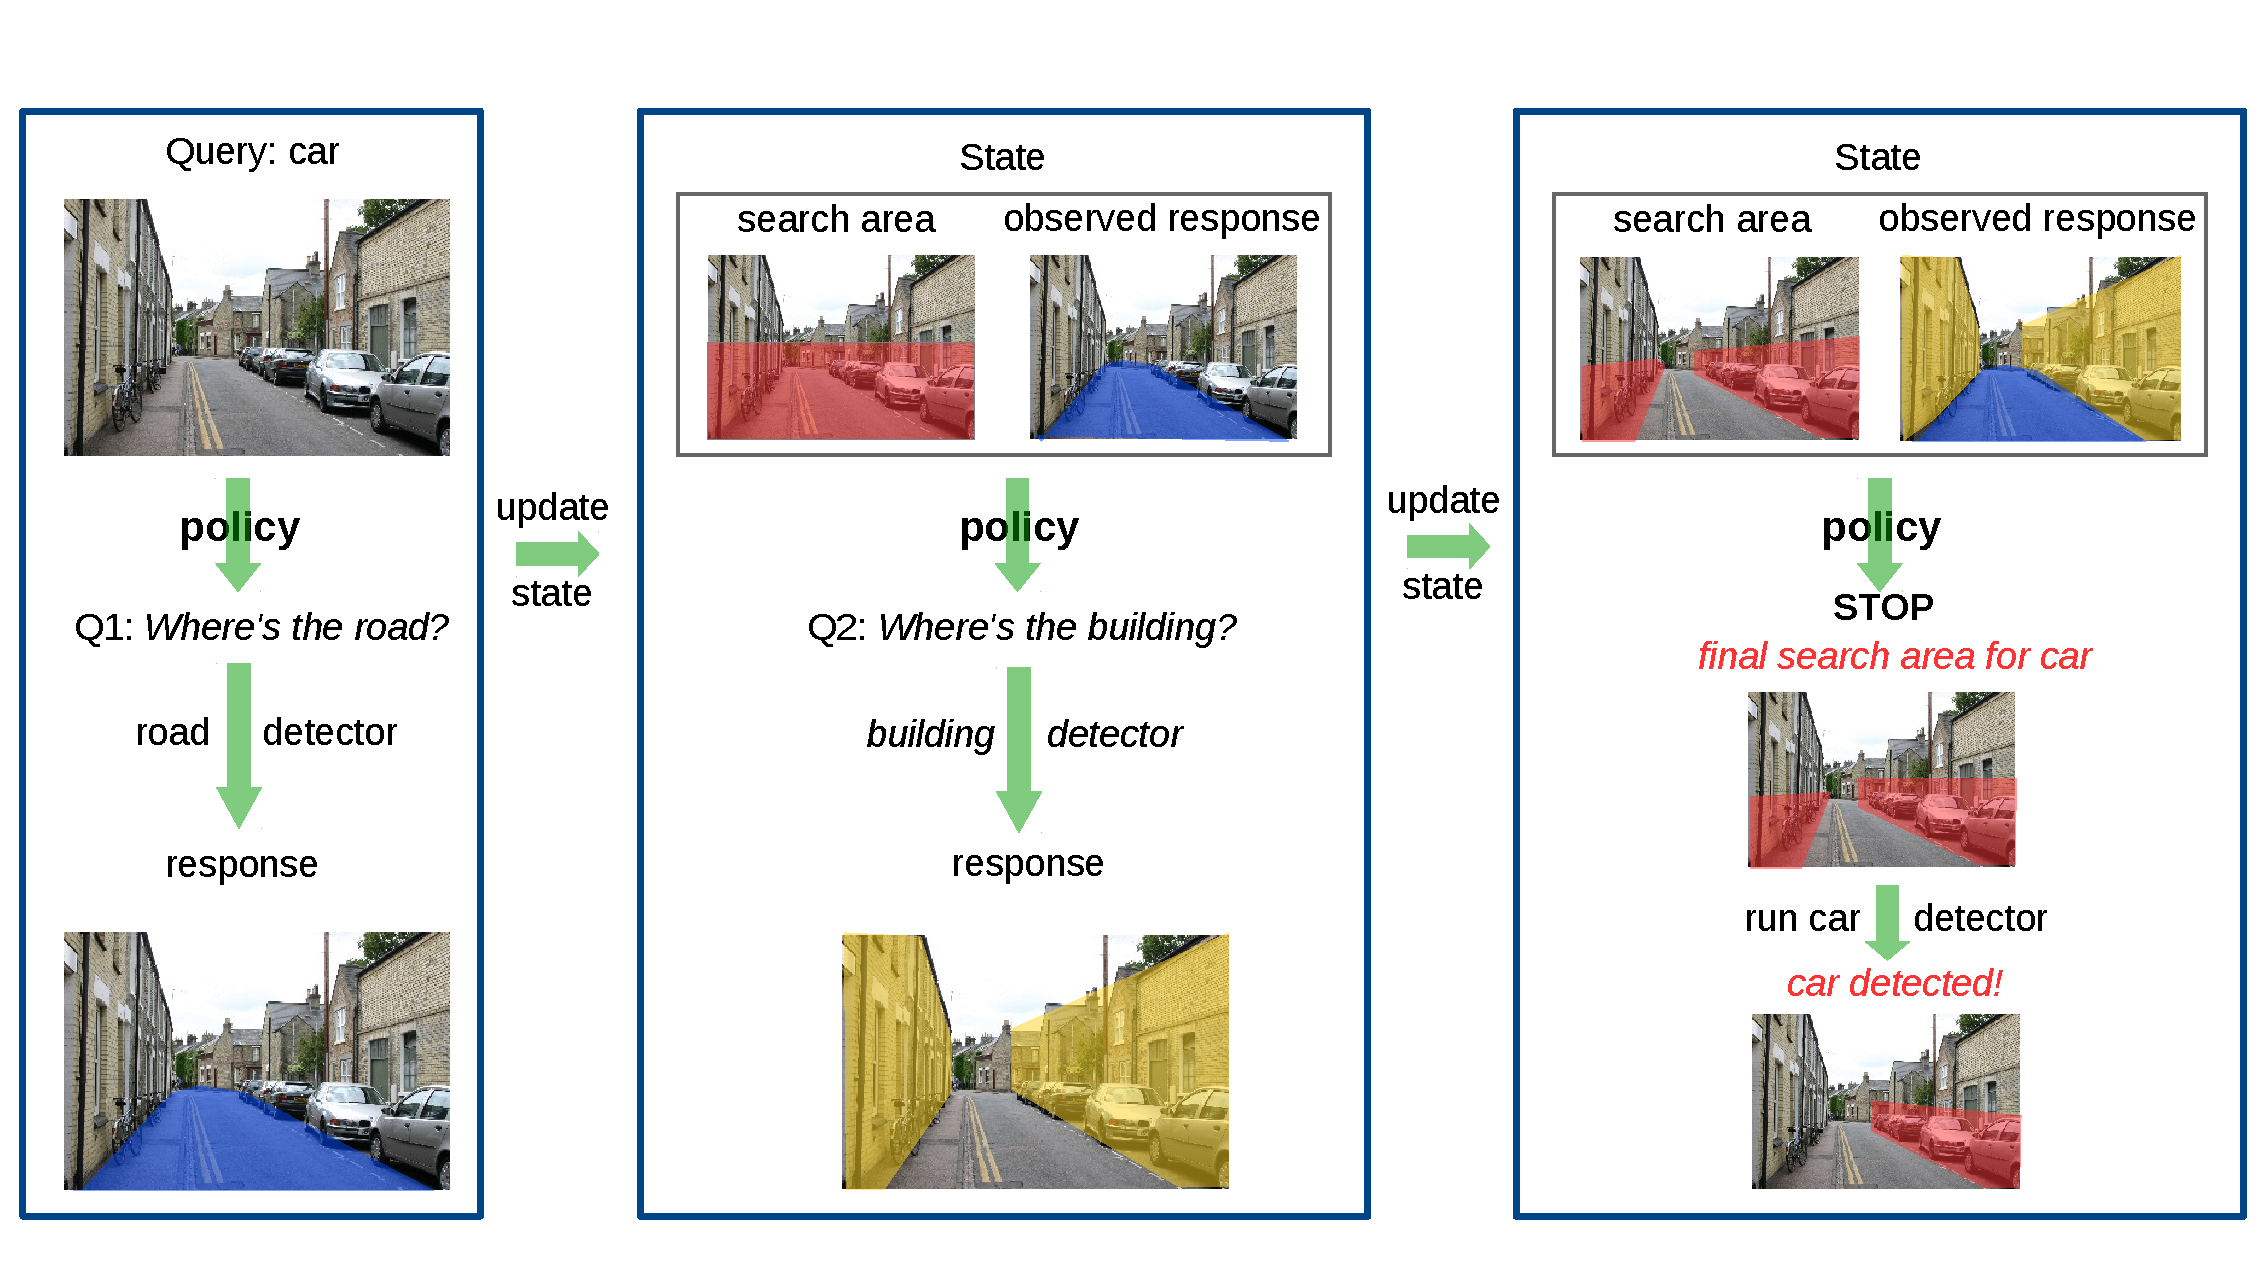
\includegraphics[width=\linewidth]{figures/iccv20q-overview.pdf}
\vspace{-1em}
\caption{Illustration of our sequential search for query objects in 20 context-driven questions.}
\label{fig:20Qintro}
\end{center}\vspace{-2em}
\end{figure*}

% The main contributions of the paper are:
% \HHNote{seems contribution 1 and 2 can be combined, they are both novelty of a new learning algorithm to the problem. e.g., we formulate and learn...}
% \begin{itemize}
% \item a novel formulation of the object detection problem as a Markov Decision Process and a dynamic, closed-loop policy learned by imitation learning to decide which detectors to run next and where to look for the query object iteratively
% \item a general and unified probabilistic framework incorporating responses from multi-class object detectors and contextual classifiers to update the search area for the target
% \item a data-driven context model that not only encodes co-occurrence but also spatial relations by efficient weighted vote maps from exemplars\HHNote{This is not explained before and it's hard to understand here what the context model is}.
% \end{itemize}





\section{Related Work}
\label{sec:relatedwork}

{\bf{Sequential Testing}}. 
The ``20 question'' approach to pattern recognition dates back to Blanchard and Geman~\cite{blanchard2005hierarchical}, motivated by the scene interpretation problem with a large number of possible explanations. Their work provides a theoretical foundation for the design of sequential algorithms. ``20 questions" approaches recently have been used to generating questions for users in applications such as image binary segmentation~\cite{rupprecht2015image} and ``visual Turing test''~\cite{geman2015visual}. But such methods involve humans in the loop during test time, which is expensive and hard to scale up.  There have been recent attempts to model the computational processes of visual attention~\cite{ranzato2014learning, larochelle2010learning} for object recognition. Such methods focus on low level salience and are tested in simple scenario such as MNIST dataset. 

There are several models~\cite{gao2011active} of objects classification that operate by running classifiers sequentially in an active order.~\cite{branson2010visual} proposed an information gain based approach to iteratively pose questions for users and incorporate human responses and computer vision detector results for fine-grained classification.
~\cite{sergey2012timely} formulated object classification as a Markov decision process to select classifiers under certain time constraints. However, these approaches only focus on classifying objects. They have not addressed the challenging problem of simultaneous segmentation and localization of objects in a multi-class scene as we do in this paper, and did not exploit inter-object spatial context.



{\bf Object Detection}. 
A common approach to object detection is based on applying gradient based features over densely sampled sliding windows~\cite{felzenszwalb2010object}.Such methods achieve good results on classes like human and vehicles, but they are very inefficient since they evaluate up to hundreds of thousands of windows in an image, and false positve detections arise. To reduce the number of windows evaluated,  category independent object proposals~\cite{carreira2012cpmc,van2011segmentation,arbelaez2014multiscale} have been proposed which generate a small number of high quality regions or windows that are likely to be objects. These approaches dramatically reduce the number of candidates and reduce false positive detections. Using these object proposals~\cite{girshick14CVPR, BharathECCV2014} train and apply deep neural network models on large datasets to learn the feature extractor and classifiers, and achieve state-of-the-art performance on the Pascal VOC detection challenge. However, such category independent proposals do not adapt to different query classes and still lead to a significant amount of unnecessary detector computation. 

{\bf Object Recognition using Context}. 
Context has been shown to improve object recognition and detection. In~\cite{gould2009decomposing, shotton2006textonboost, ladicky2010graph}, CRF models are used to combine unary potentials based on visual features extracted from superpixels with neighborhood constraints and low level context. Inter-object context in the scene has also been shown to improve recognition~\cite{galleguillos2010context, chen2011piecing}.~\cite{mottaghi2014role} shows that using contextual information can improve object detection using CRF models. However these approaches need to evaluate the high order co-occurrence statistics with \emph{all} other object classes appearing in the scene altogether, some of which may not be informative. Our framework, in contrast, only needs to evaluate the most related context in an active sequence before classifications of all objects are made, and goes beyond simple co-occurence statistics.~\cite{bogdan2012context} applied a sequential decision making framework to window selection by voting for the next window. However, the voting process needs to look up nearest neighbors in hundreds of thousands of exemplar window pairs in the training set because their context is purely based on appearance similarity at the instance level, which is highly inefficient. By contrast, our model is based on context between semantic classes so we do not compute nearest neighbors over hundreds of thousands of windows in a high dimensional descriptor space to retrieve the voters, which greatly reduces computational complexity.
% We only need votes from a few regions within the search space of context class. Our context model achieves good accuracy while greatly reducing computational complexity.

% \input{overview}
\section{Problem Formulation}
A sequential decision-making problem can be formulated as a Markov Decision
Process (MDP).
An MDP is defined by a tuple $(\mathcal{S}, \mathcal{A}, T(.), R(.))$,
where $S$ is a set of \textit{states} and $A$ is a set of
\textit{actions}. An agent interacts with the
environment by following a
\textit{policy} $\pi: S \rightarrow A$ that determines which action to take in a
given state. After taking action $a$ in
state $s$, the environment takes the
agent to the next state $s'$ according to the transition probability $T(s'|s,a)$
and responds with some reward $R(s,a)$.
Given an optimal policy $\pi^\ast$ which yields a state-action sequence that maximizes the discounted cumulative reward,
the optimal $Q$-value is recursively defined as $Q^\ast(s_t, a_t) = R(s_t, a_t) + \gamma\max_{a_{t+1}}Q^\ast(s_{t+1}, a_{t+1})$, where $a_t$ is chosen by $\pi^\ast$ and $\gamma$ is the discount factor.

Given an image $X$ and a query object class $c_q$ ($q \in {1,..,C}$),
we detect the query class of objects by sequentially making decision of exploring one context/object class, and narrow down the search area for the query based on observed responses. Our framework is shown in Figure~\ref{fig:flowchart}.
We model our problem as an MDP.
Our \textbf{state} $s_t$ is $(X, O^t)$, where  $O^t= \{o_1, o_2, ....,o_t\}$ is a sequence of observations.
The \textbf{action} set is $\{d_1, ..., d_C, \mbox{Stop}, \mbox{Reject}\}$, where $d_i$ is to run the detector of class $c_i$, ``Reject'' is to reject the query class and terminate the process\HHNote{Instead of ``terminate'', maybe say ``output not found'', I'm not sure what's the correct way to say not found in this context.}, and ``Stop'' is to run the detector of the query class on the refined search area and output the result.
The \textbf{state transition} is deterministic in our case.
We define the \textit{reward} $R$ as the immediate gain in intersection/union of the search space:
\begin{eqnarray}
\label{eq:imreward}
R(s_t,a_t) =  \frac{X^{t+1} \cap X_q}{X^{t+1} \cup X_q} - \frac{X^{t}\cap X_q}{X^{t} \cup X_q}
\end{eqnarray}
where $X^{t+1}_i$ is the updated search area after executing action $a_t$ in state $s_t$, determined by the context models described in Section~\ref{sec:context}. $X_q$ is the groundtruth mask of the query object instances in the image. 

\section{Approach}
\subsection{Learning the Policy by Imitation}
Suppose we know the optimal $Q$-values, the optimal policy is simply
\begin{eqnarray}
\label{eq:pi}
\pi^\ast(s) = \arg\max_{a\in A} Q^\ast(s,a).
\end{eqnarray}
To learn $Q^\ast$, we assume that these values are given by an oracle \emph{at training time}; thus the problem is reduced to learning
a linear approximation:
\begin{eqnarray}
\label{eq:qvalue}
Q^{\ast}(s,a) = \theta_\pi^T \phi(s,a),
\end{eqnarray}
where $\phi(s,a) = \phi((X, O^t),a) = \phi(X^t,a)$ is the feature of the underlying area $X^t$ at time $t$ after observing detector responses of $a_1,...,a_t$. 
This can be solved by standard supervised learning approaches.

The oracle's action sequence maximized the cumulative reward. Since the space of action sequences is exponential, we compute the oracle by breadth-first search with pruning. To avoid collecting examples from the oracle's trajectory only, we encourage exploration by starting from a random state.
We collect examples $(s,a,r)$ samples from the oracle's trajectory and use ridge regression to predict the Q-values.

%\section{Approach}
%
% Given an image and a query class, our algorithm detects the query class of objects by sequentially making decision of exploring one context/object class at a time, and narrow down the search area for the query based on observed responses. Our goal is to learn a policy $\pi(s)$ that can dynamically selects different sequences of ``questions''  given different query classes and images. We model the problem as an MDP and use reinforcement learning, specifically imitation learning to learn class-specific policy. 

%Under certain budget constraint, our goal is to learn a policy $\pi(s)$ that can sequentially select a contextual object class to detect  to narrow down the search area of the query or make an early rejection.  \HHNote{not sure what episode means hear..}of selecting actions for the input image $X$ and target query class $c_q$ \HHNote{$X$ and $c_q$ are not used here and they will be defined in the next section. Consider removing the notations}.

\begin{figure*}[htb]
\begin{center}
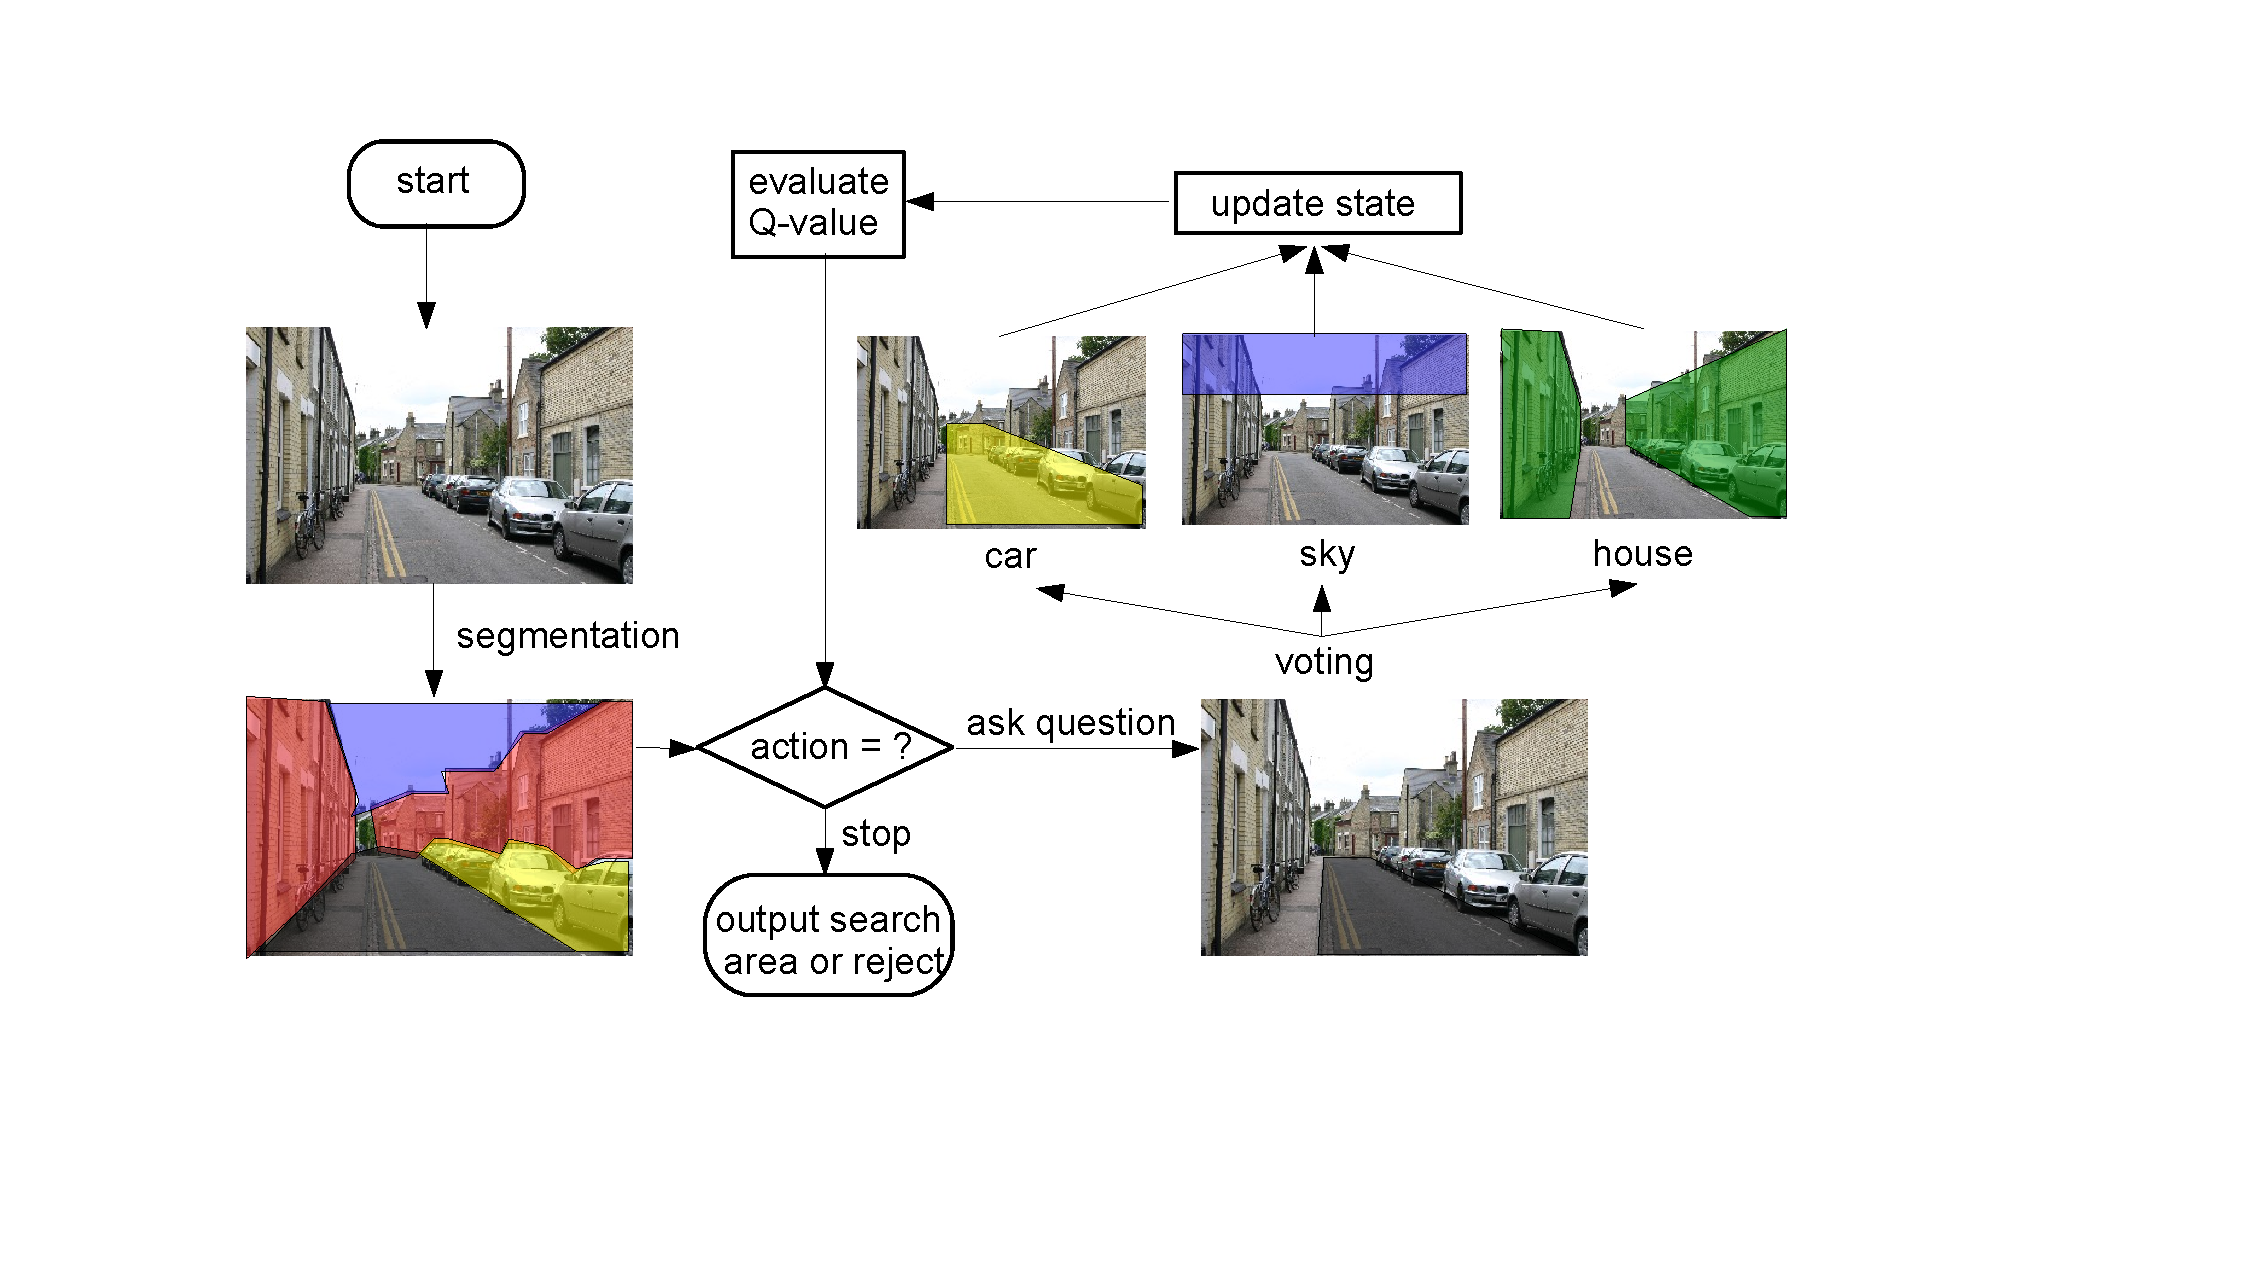
\includegraphics[width=\linewidth]{figures/flowchart_Q.pdf}
\caption{Framework of our context driven object searching. We first generate region hypotheses using object proposal algorithms, then the policy evaluates the current state and iteratively selects the action maximizing the Q-value function. Afterwards, the possible search locations are updated and the posterior probabilities of each category are evaluated for the next state.}
\label{fig:flowchart}
\end{center}

\end{figure*}

%\subsection{Object Detection as Markov Decision Process (MDP)}
%\label{sec:policy}
%
%Specifically, given an image $X$ and a query object class $c_q$ in classes ${1,..,C}$, we define the MDP as follows.
%\begin{mydef}
% The \textbf{detection action selection MDP} is defined by the tuple $(\mathcal{S}, \mathcal{A}, T(.), R(.), \gamma)$:
%\begin{itemize}
%\item \textbf{State} $s(t) = (X, O^t)\in \mathcal{S}$ that includes the image $X$ and the observations $O^t= \{x_1, x_2, ....,x_t\}$ over time till $t$. %  \HHNote{I would give some explanation of what state is before the math, e.g. a state contains necessary information for decision making}
%\item The set of \textbf{actions} to be taken in each state $\mathcal{A} = \{a_1, ..., a_C, \mbox{Stop}, \mbox{Reject}\} $, where $a_i$ is to run the detector of class $c_i$, \textit{Reject} to reject query class in the image and terminate the process, and \textit{Stop} to output the search area and run query detector.
%\item \textbf{State transition} function $T(s'|s,a, X)$ is the probability taking the agent to the next state $s'$ from $s$ by action $a$, depending on the instance $X$
%\item The \textbf{reward} function $R(s,a,s') \rightarrow \mathbb{R}$ gives reward to taking action $a$ at state $s$ to the next state $s'$
%\item The \textbf{discount} constant $\gamma$ defines a tradeoff between taking the action by greedily maximizing the immediate reward or the considering the long term expected reward.
%\item The \textbf{policy} $\pi(s): \mathcal{S} \rightarrow \mathcal{A}$ is a mapping from a state to an action.
%\end{itemize}
%\end{mydef}
%
%During test time, our search policy  iteratively selects an action $a^t \in \mathcal{A}$. Then the policy obtains response $x_t$ at time step $t$ given by the detection or classification results of action $a_t$. 
%
%\HHNote{The causal relation ``since ... we want ... then define a policy'' here doesn't seem to be right. Policy and Q-value are defined by the MDP.} 
%Formally, since we would like to select the actions dynamically, we want to learn a value function taking action $a$ in state $s$ under the policy $\pi$, denoted $Q^\pi(s,a): S\times A \rightarrow \mathbb{R}$, where $S$ is the space of all possible states, to assign a value to a potential action $a\in A$ given the current state. We can then define policy $\pi$ to take the action that maximizes the expected value:
%
%\begin{eqnarray}
%\label{eq:pi}
%\pi(s) = \arg\max_{a_i\in A\backslash R} Q(s,a_i)
%\end{eqnarray}
%
%\subsection{Reward Function}

%at each time step $t$, we select a question $q_t$ and take action $a_t$ to evaluate it. Let $R^t = \{r_1, r_2, ....,r_t\}$ be the observations of responses to the actions taken at time $1...t$, where the response $r_t = p(c_t|X)$ is the detection or classification probability of class $c_t$ corresponding to question $q_t$. 


%The parameters $\theta_\pi$ are learned by \textit{policy iteration}. We collect $(s,a,r,s')$ samples by running episodes starting from a random or empty state, then we search and prune in the tree of states and collect states samples  and corresponding features. To prevent overfitting, an $L_2$ regularized regression is trained for each class to predict the Q-values given current states.

\subsection{Context Modeling}
\label{sec:context}
Since our task is not only to detect the object but also refine the search space of the query in the image as accurately as possible, conventional modeling of context as simple co-occurrence statistics is inadequate. Instead we present a data-driven location aware approach to represent the spatial correlation between the objects and the scene. 

Given an action $a_t$ to detect context class $c_t$ at time $t$, $X_c \subset X$ is the exploration area for context, here we formulate the context $p(c|c_t,X)$ as a posterior of the probabilistic vote map $p(c_t|c,X_c)$ defined on each pixel $(x_i,x_j)\in X$ over the image, and the responses of class $c_t$ after action $a_t$:
\begin{eqnarray}
p(c_t|c,X) = \sum_{X_c \subset X} p(c|c_t,X_c)p(c_t|X_c)
\end{eqnarray}

Given a refined search space $X_c\in X$ of a context class $c_t$ at time $t$, we formalize $p(c|c_t,X)$ as a weighted vote from the cooccurring region pairs of class $c_t$ and $c$ in training scenes. Let $(s_{c_t}^i, s_c^i)$ be the $i$-th pair of co-occurring regions of class $c_t$ and $c$, and $b_{c_t}^i$ and $b_c^i$ be the corresponding bounding boxes. We can now define the probabilistic vote map $p(c|c_t,X)$ as:
\begin{eqnarray}
\label{eq:votemap}
p(c|c_t,X_c)_{s\in X^t} = \frac{1}{Z_c}\sum_i W(s_{c_t}^i,s;\theta^W).T(b_{c_t}^i,b_c^i)
\end{eqnarray}
where $s\in X^t$ is a region within the search space of the context class $c_t$. $Z_c$ is the normalization function. $W(.)$ is a kernel measuring similarity of region $s$ with a training region $s_i$. $T(b_{c_t}^i,b_c^i)$ models the transformation from $b_{c_t}^i$ to $b_c^i$, including translation and scaling. Figure~\ref{fig:votemap} shows a few examples of the vote maps. We can see that with the exemplar based and semantically aware voting, the resulted vote maps give more accurate search area of the query objects.


\begin{figure}[ht!]
\begin{center}
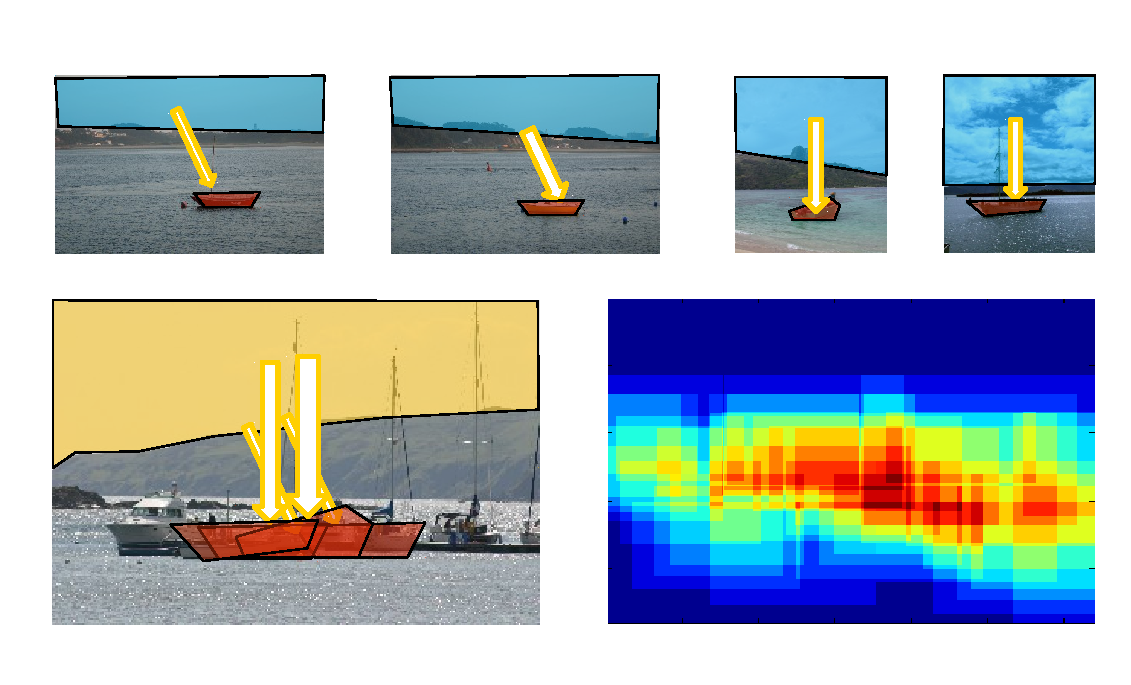
\includegraphics[width=0.6\linewidth]{figures/vote_sky_boat.pdf}
\end{center}
\caption{Examples of our weighted vote map for the context from sky to boat. The first rows are the training sample pairs of sky and boat and the second row is the test image and the resulted weighted voting map. The widths of the arrows denote the weighted similarity $W(s_{c_t}^i,s;\theta^W)$ between the test segment of sky (highlighted in yellow) and a training instance of sky segment (in light blue)}
\label{fig:vote_sky_boat}
\end{figure}


\begin{figure}[ht!]
\begin{center}
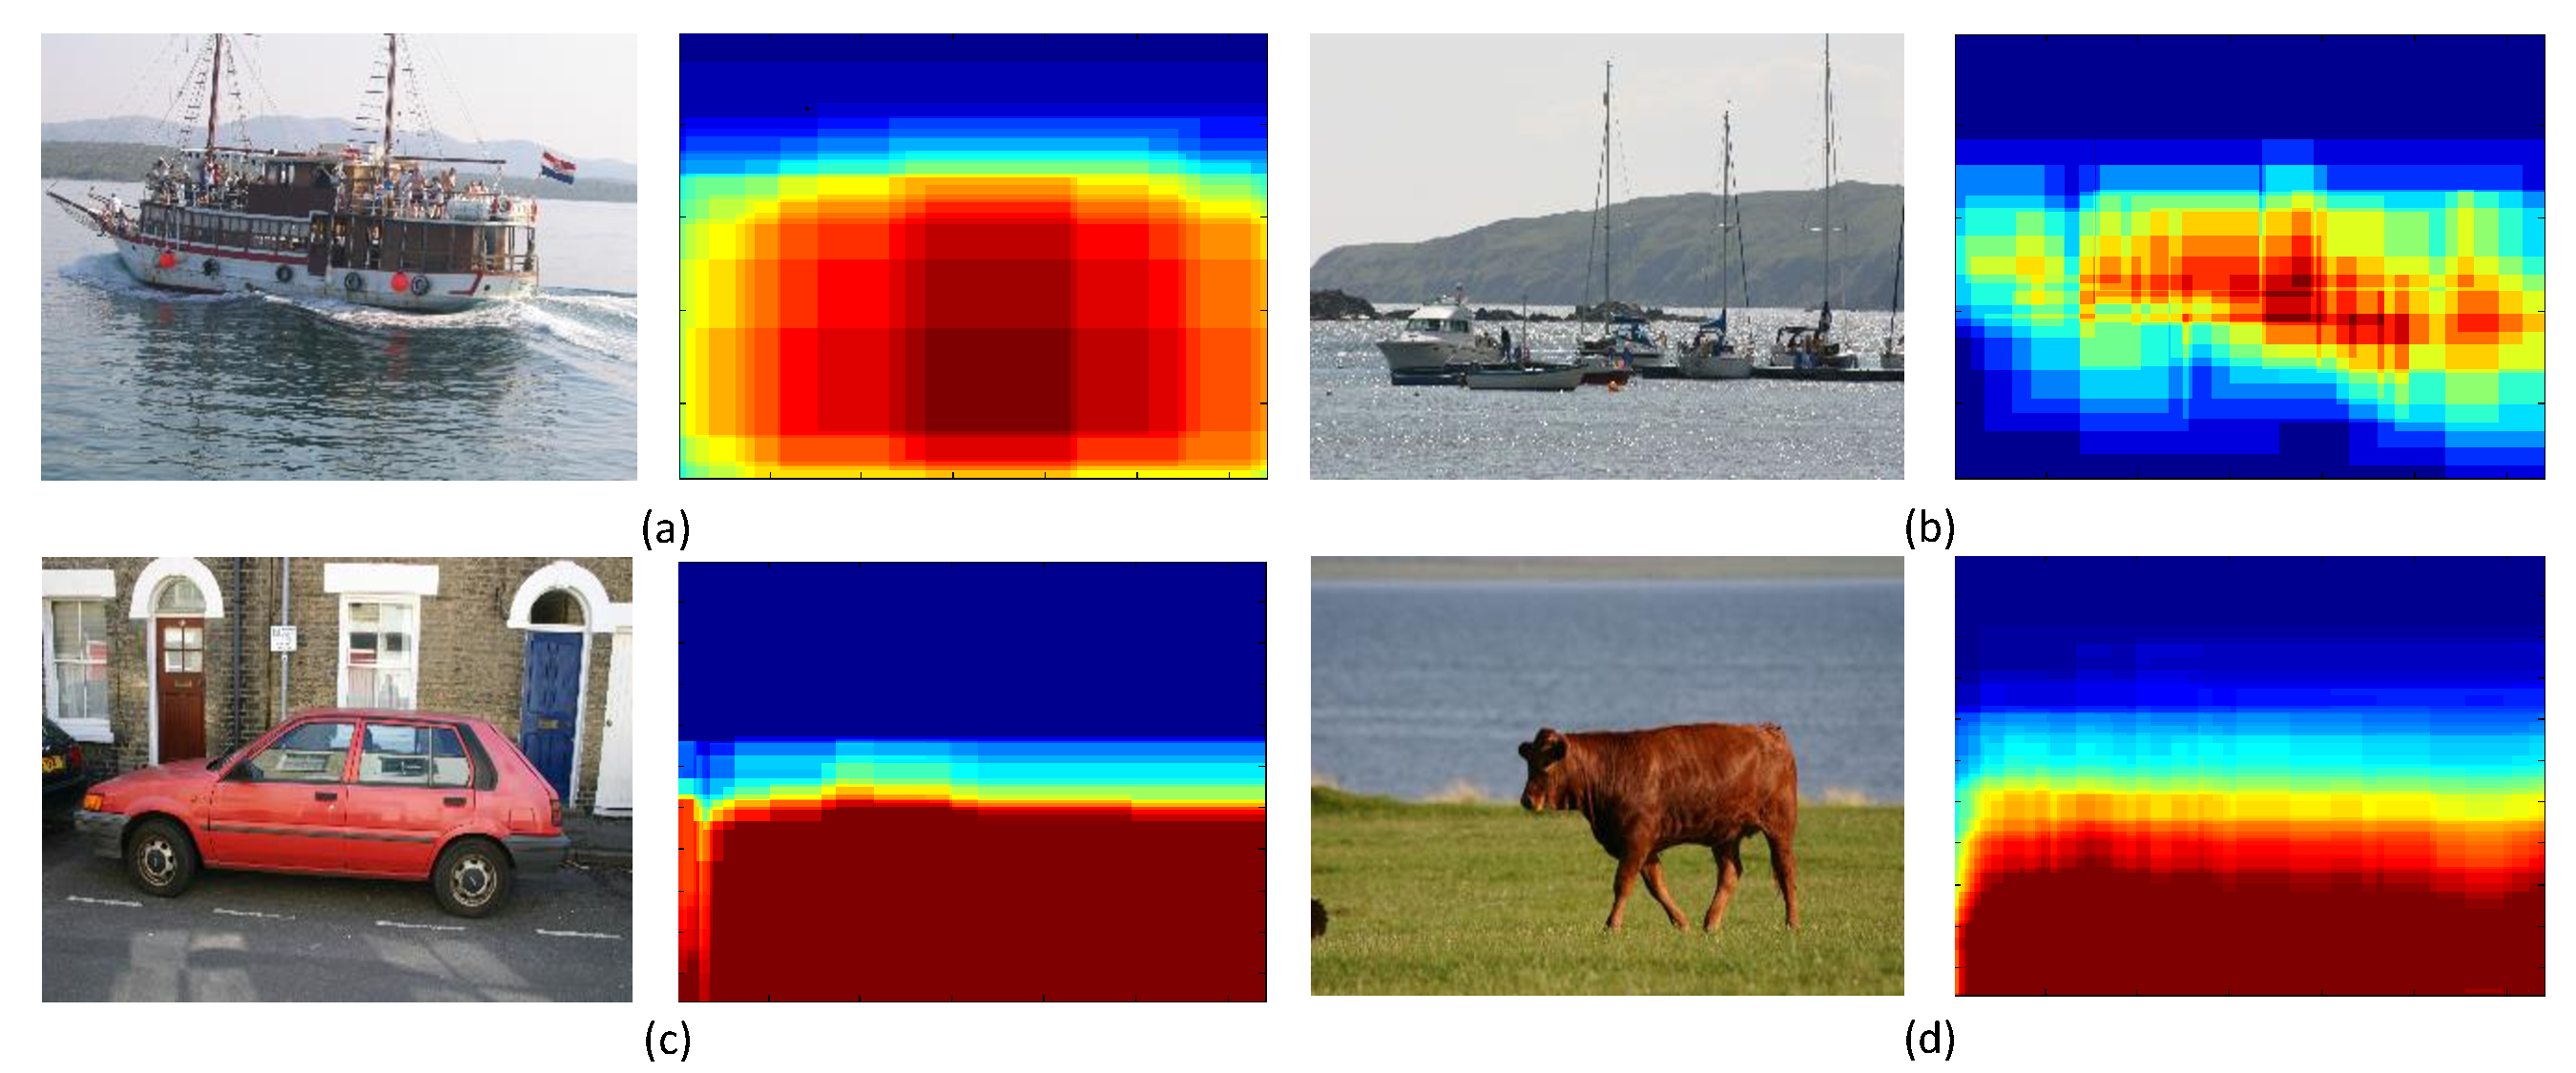
\includegraphics[width=0.6\linewidth]{figures/votemap.pdf}
\end{center}
\caption{Examples of our context vote maps. Each pair of images corresponds to the original image and the vote-based probability map of object location from observed context. From (a) - (d) are the vote maps from water to boat, sky to boat, road to car and grass to cow, respectively. Best viewed in color.}
\label{fig:votemap}
\end{figure}



The final context probabilistic vote map is given by
\begin{eqnarray}
p(c_t|c,X) = \sum_{s\in X_c} p(c_t|X_c)\sum_i W(s_{c_t}^i,s;\theta^W).T(b_{c_t}^i,b_c^i)\nonumber\\
\end{eqnarray}
where $p(c_t|X_c)$ is the probabilities of $s$ as class $c_t$ after taking the action $a_t$ to run classification at time $t$.


\subsection{Update Responses and Search Area}
After taking action $a_t$ and receiving response $o_t = p(c_t|c, X)$ from context class $c_t$, we integrate the response into observations from previous sequence of actions. Assuming the detectors and context classifiers are trained independently per category, the aggregated responses can be modeled as:
\begin{eqnarray}
p(O^t|c, X) = \prod_t p(c_t|c,X)
\end{eqnarray}

We then update the search area for the query class $c_q$ in a probabilistic framework:
\begin{eqnarray}
p(c_q|X,O^t) = \frac{p(O^t|c_q,X)p(c_q|X)}{Z}
\end{eqnarray}
where $Z = \sum_c^{C^t} p(O^t|c,X)p(c|X)$ is the normalization function, $p(c|X)$ is obtained by taking actions and running context classifiers over the context segments,  and $C^t = \{c_1, c_2, ..., c_t, c_q\}$ are the set of observed contextual classes.

% \section{Implementation Details}
\subsection{Object Proposals}
We use MCG object proposals in~\cite{arbelaez2014multiscale} as object candidates. Since the object proposals mainly covers the objects,  we also generate a small amount (20$\sim$30 per image) of segments using stable segmentation algorithm in~\cite{chen2011piecing} to cover the whole scene including contextual classes. To reduce the computation overhead, our context voting step uses only the stable segments. The stable segmentation gives a coarse level of object/context division and reduces the computation complexity of context voting compared to the large number of finer object proposals, while still maintains a semantically reasonable context inference. 

\subsection{Datasets}
We conduct our training and experiments on the Pascal VOC dataset.~\cite{Everingham10} which is a \textit{de facto} benchmark for object detection for years. Since the original dataset does not provide annotation of segmentation and contextual classes, we train our policy using the Pascal Context dataset~\cite{mottaghi2014role} which fully annotates the every pixel of the Pascal VOC 2010 train and validation sets, with additional contextual classes, which is perfectly good for our task. We use the 33 context classes and train our policy on the Pascal Context training set, and test our algorithm and baselines on the validation set. We also test our policy on the MSRC dataset~\cite{shotton2006textonboost} to show our algorithm can generalize to different data. 

\subsection{Feature Representation}
To classify the object proposals, we extract region features and classify them for object classes using the deep neural network model in~\cite{BharathECCV2014} fine-tuned on Pascal VOC 2012. For the policy action classifiers, we also use the same model to extract features for states, which concatenate the SDS features of the search areas for the query and observed context. For context classifiers we use a subset of the appearance features for superpixels from~\cite{tighe2010superparsing} and learn one-vs-all SVM models for classification.

\section{Experiments}

\subsection{Reduction of Number of Object Proposals}

Figure~\ref{fig:mapVSnumprop} shows that our 20 questions detection algorithm can effectively reduce a large amount of object proposals ($30\% \sim 40\%$) while maintaining similar mAP performance compared to exhaustive detection on all object proposals.  

\subsection{Comparison with other context based methods}

\subsection{Comparison with random search methods}


% ferrarri 2012
~\cite{bogdan2012context} 25000 to 100 
% \section{Conclusion}
We proposed a sequential and dynamic process for object detection and segmentation, in which a policy iteratively selects a context related question adapting to different query and responses from previous context-related questions, then more accurately refines the search area or rejects the object early without running many detectors. Thus it can significantly reduce computational cost while preserving good accuracy for the query class. We formulate the object detection problem as a Markov Decision Process to learn a policy by imitation learning. We present a unified probabilistic framework to model spatial context between objects. We applied this active detection scheme to the problem of object detection and segmentation, and achieved comparable or even higher average precision compared to previous approaches, but with significant computational savings. 






{\small
\bibliographystyle{ieee}
\bibliography{nips2015}
}

\end{document}
